
\chapter{Electric Charge and Electric Field}

\subsection{Electric Charge}
\textbf{Electromagnetism} (EM) affects only charged particles, mainly electrons and protons. All particles have charges that are integer multiples of the elementary charge $e$ such that the charge is given by
\begin{equation}
q = ne,
\end{equation}
where $q$ represents charge (C), $n$ represents an integer, and $e = \SI{1.6022e-19}{C}$ represents the elementary charge.

Electric charge is conserved. This means that the total charge of any isolated system with no charge moving in or out stays the same|charge is never created or destroyed. 

\textbf{Coulomb's Law} states that charges of the same sign repel and charges of the opposite sign attract. Furthermore, the force $F$ produced by charges can be calculated via
\begin{equation}
F = k\frac{q_1q_2}{r^2},
\end{equation}
where $k = \SI{9.0e9}{\frac{N m^2}{C^2}}$, $q_1$ represents the first charge, $q_2$ represents the second charge, and $r$ represents the separation distance.

The \textbf{principle of superposition of forces} is the vector sum of the individual forces
\begin{equation}
F = k\frac{q_1q_2}{r_{12}^2}r_{12} + k\frac{q_1q_2}{r_{13}^2}r_{13} = q_1 \vec{E}
\end{equation}
\newpage

\subsection{Electric Field and Electric Forces}

The \textbf{electric field of a point charge} can be calculated using the following formula:
\begin{equation}
\vec E (\vec r_0)= \frac{kq}{r^2} = \frac{\vec{F}}{q}
\end{equation}
where, $q$ denotes the charge of the point source (C) and $r$ denotes the radial distance of the point charge from the origin.

The \textbf{electric field of an group of charges} is the superposition of all the electric forces from all the charges. This can be approximated with volume charge density ($\rho$) via
\begin{equation}
\vec{E}(\vec{r_o}) = \frac{1}{4\pi \epsilon_0} \int\frac{\rho(\vec{r}) (\vec{r_0} - \vec{r})}{\abs{\vec{r_0} - \vec{r}}^3} \di x \di y \di z,
\end{equation}

where $\epsilon_0 = \SI{8.854e-12}{\frac{C^2}{N \cdot m^2}}$, $\rho(\vec{r})$ is the surface charge density, and $\vec{r}$ is the radius.

For \textbf{a conductor without current flow}, the charge all resides on the surface. To approximate the electric field, we can use surface charge density $\sigma (\vec{r})$
\begin{equation}
\vec{E}(\vec{r_o}) = \frac{1}{4\pi \epsilon_0} \int\frac{\sigma(\vec{r}) (\vec{r_0} - \vec{r})}{\abs{\vec{r_0} - \vec{r}}^3} \di A,
\end{equation}

If one has a \textbf{thin wire} where all the charge resides, with linear charge density $\lambda(\vec{r}) = \frac{\di q}{\di l}$, where $\di l$ is the element of length along the wire, then

\begin{equation}
\vec{E}(\vec{r_o}) = \frac{1}{4\pi \epsilon_0} \int\frac{\lambda(\vec{r}) (\vec{r_0} - \vec{r})}{\abs{\vec{r_0} - \vec{r}}^3} \di l,
\end{equation}

\subsection{Electric Field Lines}
Electric field lines have tangent vectors parallel to the electric field and begin only on positive charges and end only on negative charges, though they can also go to infinity in either direction

\newpage
\subsection{Electric Dipoles}
An \textbf{electric dipole} is a pair of point charges of equal magnitude and opposite sign (a positive charge $q$ and a negative charge $-q$ separated by a distance d.

And \textbf{electric dipole moment} is the product of the positive charge $q$ and the displacement $d$ it is separated from the negative charge $-q$,
\begin{equation}
\vec{p} = q\vec{d}
\end{equation}
To approximate the electric dipole of a huge number of elementary charges (total charge is neutral), we can use the volume charge density formula $\rho(\vec{r}) = \rho(x\vec{i} + y\vec{j} + z\vec{k}) = \rho(x, y, z) $ in the following formula
\begin{equation}
\vec{P} = \int\rho(\vec{r})\vec{r}\di x \di y \di z
\end{equation}
The total force on an electric dipole is just the net force from an external electric field (the electric field from all the other charges that are not part of the electric dipole). This is true for the total torque.

If the electric dipole moment $\vec{P}$ is not parallel to $\vec{E}$, then the electric field exerts a torque on the dipole which can be calculated using
\begin{equation}
\vec{\tau} = \vec{P} \times \vec{E}
\end{equation}
where, $\vec{P}$ is the electric dipole moment, $\vec{E}$ is the electric field, and the direction of $\tau$ is perpendicular to both $\vec{P}$ and $\vec{E}$

To calculate the potential energy pf a dipole, you can use the following formula
\begin{equation}
U = -\vec{P}\cdot \vec{E}
\end{equation}

To approximate the field of an electric dipole at $r>>d$ and using binomial expansion, we can use the following formula
\begin{equation}
\vec{E}(\vec{r}) = \frac{3(\vec{p}\cdot \vec{r})(\vec{r} - \vec{p})}{4 \pi \epsilon_0 r^3}
\end{equation}
where $\vec{p} = p\cos(\theta)$, and $\epsilon_0 = \SI{8.854e-12}{\frac{C^2}{N \cdot m^2}}$

%\begin{figure}[h]
%    \centering
%    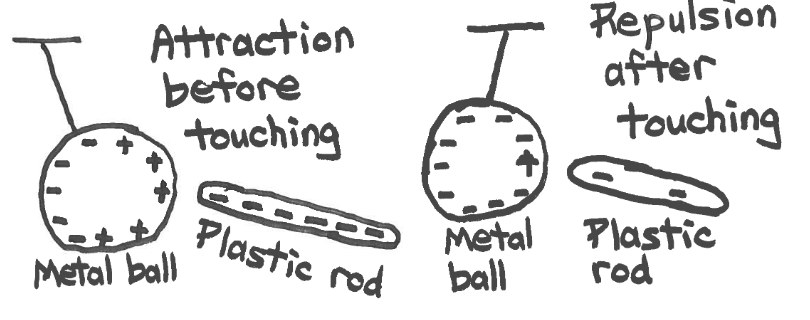
\includegraphics[width = 0.5\linewidth]{chapter1_conductors.png}
%    \caption{Image of charging by conduction}
%    \label{figure:1} 
%\end{figure}
